\documentclass[tikz,border=2pt]{standalone}

\usepackage{amsmath}
\usepackage{pifont}  % for \ding symbols
\usepackage{xcolor}
\usepackage{tikz}
\usetikzlibrary{arrows.meta,positioning,fit,backgrounds,calc,decorations.pathreplacing,patterns,shapes.geometric}
\usepackage{pgfplots}
\pgfplotsset{compat=1.18}
\usepgfplotslibrary{groupplots,fillbetween}

% ── Color palette (NeurIPS-style, colorblind-friendly) ──
\definecolor{bestcolor}{HTML}{E8F5E9}
\definecolor{gaincolor}{HTML}{1B5E20}
\definecolor{cStandard}{HTML}{BF616A}   % muted red
\definecolor{cAOI}{HTML}{5E81AC}        % steel blue
\definecolor{cDelta}{HTML}{A3BE8C}      % sage green
\definecolor{cVisual}{HTML}{D08770}     % muted orange
\definecolor{cASR}{HTML}{B48EAD}        % muted purple
\definecolor{cNarr}{HTML}{88C0D0}       % light blue
\definecolor{cAccent}{HTML}{EBCB8B}     % warm yellow
\definecolor{cGray}{HTML}{4C566A}       % dark gray
\definecolor{cLightGray}{HTML}{D8DEE9}  % light gray

\begin{document}
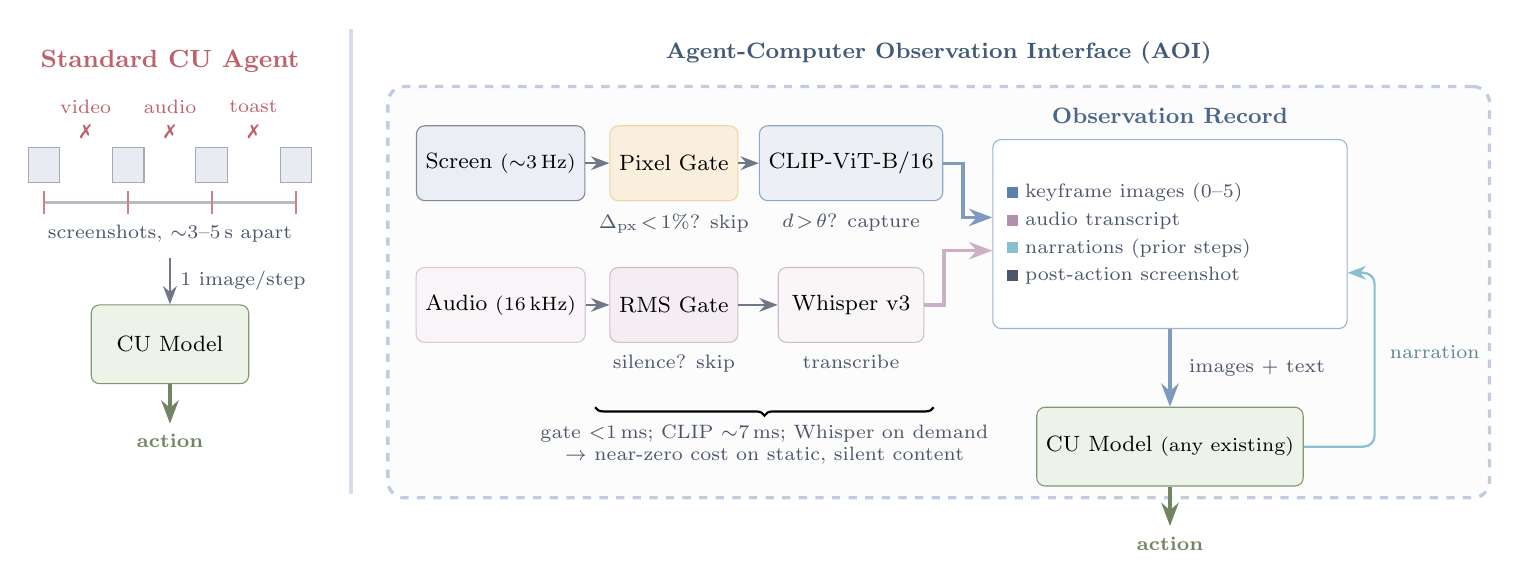
\begin{tikzpicture}[
    >=Stealth,
    box/.style={draw, rounded corners=3pt, minimum height=0.95cm, align=center, font=\footnotesize},
    env/.style={box, fill=cLightGray!50, draw=cGray!70, minimum width=1.6cm},
    gate/.style={box, fill=cAccent!30, draw=cAccent!80, minimum width=1.55cm},
    proc/.style={box, fill=cAOI!12, draw=cAOI!70, minimum width=1.85cm},
    obs/.style={box, fill=white, draw=cAOI!60, minimum width=4.5cm, minimum height=2.4cm},
    mdl/.style={box, fill=cDelta!18, draw=cDelta!80!black, minimum width=2.6cm, minimum height=1cm},
    arr/.style={->, thick, cGray!80},
    harr/.style={->, very thick, cAOI!80},
    lbl/.style={font=\scriptsize, text=cGray},
  ]
  % ── Left: Standard CU Agent ──
  \node[font=\small\bfseries, text=cStandard] at (1.6, 4.2) {Standard CU Agent};

  % Timeline with screenshots
  \draw[thick, cGray!40] (0, 2.4) -- (3.2, 2.4);
  \foreach \x in {0, 1.07, 2.13, 3.2} {
    \draw[thick, cStandard!80] (\x, 2.25) -- (\x, 2.55);
    \draw[cGray!50, fill=cLightGray!60] (\x-0.2, 2.65) rectangle (\x+0.2, 3.1);
  }
  \node[font=\scriptsize, text=cGray] at (1.6, 2.0) {screenshots, $\sim$3--5\,s apart};

  % Blind gaps with X marks
  \foreach \x/\t in {0.53/video, 1.6/audio, 2.66/toast} {
    \node[font=\scriptsize, text=cStandard] at (\x, 3.30) {\ding{55}};
    \node[font=\scriptsize, text=cStandard] at (\x, 3.62) {\t};
  }

  % Model
  \node[mdl, minimum width=2.0cm] (sm) at (1.6, 0.6) {CU Model};
  \draw[arr] (1.6, 1.7) -- (sm.north) node[midway, right, lbl] {1 image/step};
  \draw[arr, cDelta!70!black, very thick] (sm.south) -- ++(0,-0.5)
    node[below, font=\scriptsize\bfseries, text=cDelta!70!black] {action};

  % ── Divider ──
  \draw[very thick, cLightGray] (3.9, -1.3) -- (3.9, 4.6);

  % ── Right: AOI Pipeline ──

  % Input streams
  \node[env] (scr) at (5.8, 2.9) {Screen {\scriptsize($\sim$3\,Hz)}};
  \node[env, fill=cASR!10, draw=cASR!50] (aud) at (5.8, 1.1) {Audio {\scriptsize(16\,kHz)}};

  % Gates
  \node[gate] (pg) at (8, 2.9) {Pixel Gate};
  \node[gate, fill=cASR!15, draw=cASR!60] (rg) at (8, 1.1) {RMS Gate};

  \draw[arr] (scr) -- (pg);
  \draw[arr] (aud) -- (rg);

  % Gate sublabels (between rows; tight to box)
  \node[font=\scriptsize, text=cGray, anchor=north, yshift=-1pt] at (pg.south) {$\Delta_\text{px}\!<\!1\%$? skip};
  \node[font=\scriptsize, text=cGray, anchor=north, yshift=-1pt] at (rg.south) {silence? skip};

  % Processors
  \node[proc] (clip) at (10.25, 2.9) {CLIP-ViT-B/16};
  \node[proc, fill=cASR!8, draw=cASR!60] (wh) at (10.25, 1.1) {Whisper v3};

  \draw[arr] (pg) -- (clip);
  \draw[arr] (rg) -- (wh);

  % Processor sublabels (between rows; tight to box)
  \node[font=\scriptsize, text=cGray, anchor=north, yshift=-1pt] at (clip.south) {$d\!>\!\theta$? capture};
  \node[font=\scriptsize, text=cGray, anchor=north, yshift=-1pt] at (wh.south) {transcribe};

  % Observation Record (further right; title above box, below AOI banner)
  \node[obs] (orec) at (14.3, 2.0) {};
  \node[font=\footnotesize\bfseries, text=cAOI!80!black, anchor=south, yshift=2pt] at (orec.north) {Observation Record};
  \node[font=\scriptsize, text=cGray, align=left, anchor=west] at (12.10, 2.00) {%
    \textcolor{cAOI}{\rule{4pt}{4pt}} keyframe images (0--5)\\[2pt]
    \textcolor{cASR}{\rule{4pt}{4pt}} audio transcript\\[2pt]
    \textcolor{cNarr}{\rule{4pt}{4pt}} narrations (prior steps)\\[2pt]
    \textcolor{cGray}{\rule{4pt}{4pt}} post-action screenshot};

  \draw[harr] (clip.east) -- ++(0.25,0) |- ([yshift=6pt]orec.west);
  \draw[harr, cASR!70] (wh.east) -- ++(0.25,0) |- ([yshift=-6pt]orec.west);

  % CU Model (placed below the Observation Record)
  \node[mdl] (cm) at (14.3, -0.7) {CU Model {\scriptsize(any existing)}};
  \draw[harr, very thick] (orec.south) -- (cm.north)
    node[midway, right=3pt, lbl] {images + text};

  % Narration feedback loop (routed around the right side)
  \draw[harr, cNarr, thick, rounded corners=4pt]
    (cm.east) -- ++(0.9,0) coordinate (narrcorner) |- ([yshift=-14pt]orec.east);
  \node (narrlabel) [font=\scriptsize, text=cNarr!70!black, anchor=west, xshift=2pt] at ($(narrcorner)+(0,1.2)$) {narration};
  \coordinate (narrfit) at ($(narrlabel.east)+(-0.35,0)$);

  % Action output
  \draw [arr, very thick, cDelta!70!black] (cm.south) -- ++(0, -0.5)
    node(action)[below, font=\scriptsize\bfseries, text=cDelta!70!black] {action};
  \coordinate (cmfit) at ($(cm.south)+(0,0.35)$);

  % Brace annotation for gates (kept to gate+processor band, two-line label)
  \draw[thick, decorate, decoration={brace, amplitude=3pt, mirror}]
    (7, -0.20) -- (11.3, -0.20);
  \node[font=\scriptsize, text=cGray, align=center, anchor=north] at (9.15, -0.30) {%
    gate $<$1\,ms; CLIP $\sim$7\,ms; Whisper on demand\\
    $\to$ near-zero cost on static, silent content};

  % ── AOI bounding box ──
  \begin{scope}[on background layer]
    \node[draw=cAOI!40, line width=1.2pt, dashed, rounded corners=6pt, fill=cAOI!2,
          inner xsep=10pt, inner ysep=14pt,
          fit=(scr)(aud)(pg)(rg)(clip)(wh)(orec)(cmfit)(narrcorner)(narrfit),
          label={[font=\footnotesize\bfseries, text=cAOI!70!black, anchor=south, yshift=4pt]above:Agent-Computer Observation Interface (AOI)}] {};
  \end{scope}

\end{tikzpicture}
\end{document}